\documentclass{article}
\usepackage[utf8]{inputenc}
\usepackage{graphicx}
%\usepackage{blindtext}
%\usepackage{tcolorbox}
\usepackage[margin=2.5cm]{geometry}
%\usepackage{bbding}
%\usepackage{pifont}
%\usepackage{float}
%\usepackage{wasysym}
\usepackage{amssymb}
\usepackage{amsmath}
\usepackage{amsthm}
\usepackage[boxed]{algorithm2e}
\usepackage{tikz}
\usetikzlibrary{arrows,chains,matrix,positioning,scopes,graphs}


\theoremstyle{definition}
\newtheorem{defn}{Definition}


\newcommand{\vektorz}[2]{\begin{pmatrix} #1 \\ #2 \end{pmatrix}}
\newcommand{\BigO}[1]{\ensuremath{\operatorname{O}\bigl(#1\bigr)}}

\begin{document}
	
\section{Encodings}
	
	In the following section, we discuss how to make use of SAT solvers when faced with concrete problems.
	A wide variety of problems can be encoded as SAT, such as (finite) arithmetic, various practical combinatorial problems, hardware and software verification problems, and planning problems.
	To solve instances of such problems with SAT solving, an appropriate encoding is required, which is by no means unique; the chosen encoding highly influences the runtime of the SAT solver.
	Consequently, a lot of research is being done on good encodings for general and particular problems; still, it often is more of an art than a science.
	
	\subsection{Basic principles}
		
	The typical application of SAT solving makes use of \emph{finite domain variables}, e.g. $x \in \{ v_1, \ldots , v_n \}$. Relationships between these variables are expressed as equality-formulas, such as $x = v_3 \Rightarrow y \neq v_2$. There are multiple ways to encode finite domain variables in propositional logic:
	\begin{itemize}
	\item \textbf{Direct encoding} or \textbf{one-hot-encoding}: Boolean variables are introduced in the form of \[x_v \Leftrightarrow\ \text{''x takes value v''}.\] As a consequence of this encoding, additional clauses are required such that each problem variable takes exactly one value from its domain (using at-most-one and at-least-one constraints which are explained later). Direct encoding needs comparably many variables, but the encoding of the their constraints is simple.
	\item \textbf{Log-encoding} or \textbf{binary encoding}: Instead of one boolean for each variable and each value, boolean variables $b_i^x$ for $0 \leq i < \lceil \log_2 n \rceil$ are being introduced in order to encode the value of each problem variable as a binary number. Each value gets assigned a binary number, e.g. \[v_1 \mapsto 00, v_2 \mapsto 01, v_3 \mapsto 10.\] Additionally, inadmissable values must be excluded (except the domain size happens to be a power of two), e.g. $x \in \{v_1, v_2, v_3\} \text{ requires } (\bar{b_0^x} \vee \bar{b_1^x})$ such that the value $11$ will not be taken. The encoding of constraints can become more complicated with binary encoding, but for large domain sizes the amount of variables will be much smaller than by direct encoding. Also note that binary encoding implicitly makes sure that each problem variable is assigned \emph{at most one} value, without any additional clauses. When excluding all inadmissable values, the encoding even ensures the existence of \emph{exactly one} value per problem variable.
	\end{itemize}
	Generally, when comparing encodings, different aspects have to be considered: not only the size (i.e. the number of variables and the number of clauses), but also the propagation properties.
	
\subsubsection{At-most-one constraints}	
	
We define an important type of constraint which is often needed for encoding practical problem instances:

\begin{defn}
\emph{AtMostOne($x_1, \ldots , x_n$)} is the constraint that no more than one variable / literal out of $x_1, \ldots , x_n$ is set to \texttt{True}.
\end{defn}

Alternative notations include $\leq 1 (x_1, \ldots , x_n)$ and $x_1 + \ldots + x_n \leq 1$ (interpreting the variables' values as 0 and 1).

To encode at-most-one constraints, a naïve approach called \emph{pairwise encoding} is to add clauses $(\bar{x_i} \vee \bar{x_j})$ for $1 \leq i < j \leq n$ which results in \[\vektorz{n}{2} = \frac{n (n-1)}{2} \in \mathcal{O}(n^2)\] clauses. We can do better: 

\begin{figure}
\centering
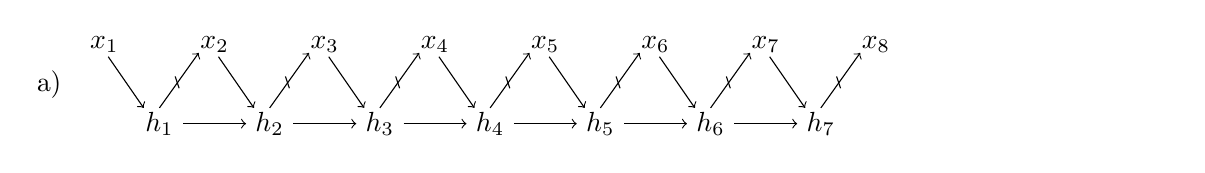
\begin{tikzpicture}
\node at (-0.7,-0.5) {a)};

\pgfmathsetmacro{\n}{8}

\pgfmathsetmacro{\nmo}{\n-1}
\pgfmathsetmacro{\nmt}{\n-2}
\foreach \i in {1,...,\n} {
	\pgfmathsetmacro{\x}{(\i-1)*1.4}
	\node at (\x,0) {$x_\i$};
}
\foreach \i in {1,...,\nmo} {
	\pgfmathsetmacro{\x}{(\i-1)*1.4+0.7}
	\node at (\x,-1) {$h_\i$};
	
	% arrows x_i -> h_i
	\draw[->] (\x-0.65,-0.15) to (\x-0.2,-0.8);

	% strikethrough arrows h_i -> x_2
	\draw[->] (\x,-0.8) to (\x+0.5,-0.1);
	\draw (\x+0.2,-0.4) to (\x+0.25,-0.55); 
}
\foreach \i in {1,...,\nmt} {
	\pgfmathsetmacro{\x}{(\i-1)*1.4+0.7}
	% arrows h_i -> h_{i+1}
	\draw[->] (\x+0.3,-1) to (\x+1.1,-1);
}

\node at (13.5,-1) {\ };
\end{tikzpicture}\\ \vspace*{0.5cm}
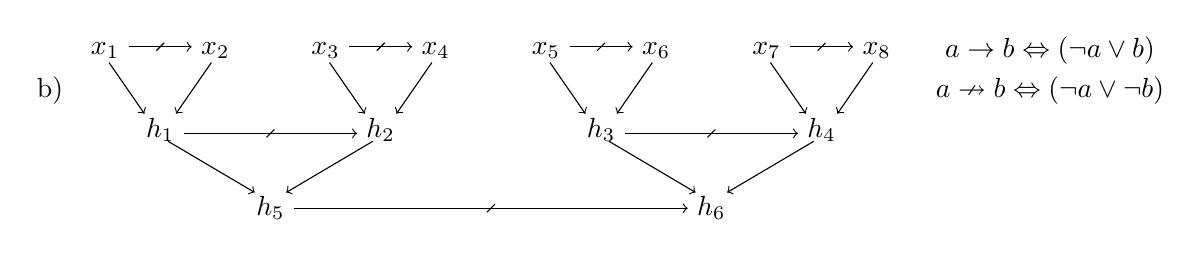
\begin{tikzpicture}
\node at (-0.7,-0.5) {b)};

\pgfmathsetmacro{\n}{8}

\pgfmathsetmacro{\nh}{0.5*\n}
\pgfmathsetmacro{\nq}{0.25*\n}

\foreach \i in {1,...,\n} {
	\pgfmathsetmacro{\x}{(\i-1)*1.4}
	\node at (\x,0) {$x_\i$};
}

\foreach \i in {1,...,\nh} {
	\pgfmathsetmacro{\x}{(\i-1)*2.8}
	\draw[->] (\x+0.3,0.05) to (\x+1.1,0.05);
	\draw (\x+0.75,0.1) to (\x+0.65,0.0);

	\node at (\x+0.7,-1) {$h_\i$};
	\draw[->] (\x+0.05,-0.15) to (\x+0.5,-0.8);
	\draw[->] (\x+1.35,-0.15) to (\x+0.9,-0.8);
}

\foreach \i in {1,...,\nq} {
	\pgfmathsetmacro{\x}{(\i-1)*5.6+2.1}
	\pgfmathsetmacro{\nodenum}{int(\i+4)}
	\draw[->] (\x-1.1,-1.05) to (\x+1.1,-1.05);
	\draw (\x-0.05,-1.1) to (\x+0.05,-1.0);

	\node at (\x,-2) {$h_\nodenum$};
	\draw[->] (\x-1.3,-1.15) to (\x-0.2,-1.8);
	\draw[->] (\x+1.3,-1.15) to (\x+0.2,-1.8);
}

\draw[->] (2.4,-2) to (7.4,-2);
\draw (4.85,-2.05) to (4.95,-1.95);

\node at (12,0) {$a \rightarrow b \Leftrightarrow (\neg a \vee b)$};
\node at (12,-0.5) {$a \nrightarrow b \Leftrightarrow (\neg a \vee \neg b)$};

\end{tikzpicture}
\caption{Efficient \emph{at-most-one} encodings. a) Ladder encoding; b) tree encoding. }
\label{fig:atmostone_encodings}
\end{figure}

\emph{Ladder encoding} makes use of $n-1$ additional helper variables in order to reduce the amount of necessary clauses to $3n-4 \in \mathcal{O}(n)$. We examine the graphical encoding in figure \ref{fig:atmostone_encodings} a): If one variable $x_i$ is set to \texttt{True}, the value \texttt{True} is propagated to all helper variables $h_j, j > i$, and, as a result of the negative implications $h_j \nrightarrow x_{j+1}$, all variables $x_j, j > i$ must be \texttt{False}. By contrast, the value \texttt{False} is propagated to $h_{i-1}$ because of the negative implication $h_{i-1} \nrightarrow x_i$ and forces all helper variables to the left to be \texttt{False} such that the implications $x_j \rightarrow h_j$ enforce all $x_j, j < i,$ to be \texttt{False}. So we can see that this encoding guarantees that no more than a single variable $x_i$ can be \texttt{True}.

\emph{Tree encoding} is using the same idea as ladder encoding, but uses a binary tree like structure to make use of a faster propagation of variable values. If the number of variables $x_i$ is a power of two, $n-2$ extra variables are needed and the number of clauses is $3n-5$. If it is not, some additional variables and clauses have to be added to maintain the structure of the encoding.
% (n-1)*1 + (n-2)*2 = n-1 + 2n-4 = 3n-5

\subsection{Planning}

Planning is the process of finding a plan, i.e. a sequence of actions that changes the state of the world from some initial state to a desired (goal) state. Because of the generality of this definition, there are countless examples for planning applications such as delivering some packages, building a submarine, robot motion planning or fulfilling a scientific goal by an autonomous space probe.

\begin{figure}[h]
\begin{center}
\includegraphics[width=12cm]{plan-example.pdf}
\caption{A truck delivery as an easy example for planning}
\end{center}
\end{figure}

To introduce a formal definition of planning, consider the following example of a truck with the objective to deliver certain packages:
\begin{itemize}
\item \emph{Initial State:} There is a truck and a package in city $A$, and there is a package in city $B$.
\item \emph{Goal:} There are two packages in city $C$.
\item \emph{Possible Actions:} (Un)loading packages from/on the truck and driving between cities.
\end{itemize}

Using the same terms as in that example, we define a planning problem as follows:

\begin{defn}
A \emph{planning problem instance} is a tuple $\Pi = (\mathcal{X}, \mathcal{A}, s_I, s_G)$ where $\mathcal{X}$ is a set of multivalued variables with finite domains, $\mathcal{A}$ is a set of actions where each action $a \in \mathcal{A}$ is a tuple $(\text{pre}(a), \text{eff}(a))$ of preconditions and effects, $s_I$ is the initial state (a full assignment of the variables in $\mathcal{X}$) and $s_G$ is the set of goal conditions.
\end{defn}

Each variable $x \in \mathcal{X}$ has a finite possible set of values $\textit{dom}(x)$. Preconditions, effects, the initial state and the goal conditions share the same structure; they are sets of equalities of the form $x = v$ where $x \in \mathcal{X}$ and $v \in \textit{dom}(x)$.

A \emph{state} (also: \emph{world state}) is a full assignment of the variables in $\mathcal{X}$, i.e. each variable $x \in \mathcal{X}$ has exactly one value assigned from its domain $\textit{dom}(x)$. A state can be represented as a set of equalities as just mentioned. By this definition, the initial state $s_I$ qualifies as a state itself; furthermore, a state $s$ is a \emph{goal state} if $s_G \subseteq s$, such that all of the goal conditions are met.

We call an action $a \in \mathcal{A}$ \emph{applicable} in the state $s$ if $\textit{pre}(a) \subseteq s$. When such an action is applied in the state $s$, it changes to the state $s'$ such that $\textit{eff}(a) \subseteq s'$ and the difference between $s$ and $s'$ is minimal -- only the variables used in $\textit{eff}(a)$ may be changed.

A \emph{plan} for a planning problem is a sequence of actions $P = (a_1, a_2, \ldots, a_n) \in \mathcal{A}^n$ such that $s_1 = s_I$, $a_i$ is applicable in $s_i$ and $s_{i+1} = apply(s_i, a_i)$,  and $s_G \subseteq s_{n+1}$. So a plan begins at the planning problem's initial state and then includes a number of state transitions which can occur by applicable actions. We call $n$ the length of the plan $P$. An \emph{optimal plan} is a plan of shortest possible length.\\

We can now formalize the previous trucking example. We define the variable $T$ as the truck location with $\textit{dom}(T) = \{A, B, C\}$ as well as the package locations $P_1$ and $P_2$ with $\textit{dom}(P_1) = \textit{dom}(P_2) = \{A, B, C, T\}$. Let the initial state $s_I = \{T = A, P_1 = A, P_2 = B\}$ and the goal $s_G = \{P_1 = C, P_2 = C\}$. Additionally, we define the following actions:
\begin{itemize}
\item $\textit{load}(P_i, L) = (\{T = L, P_i = L\}, \{P_i = T\})$
\item $\textit{unload}(P_i, L) = (\{T = L, P_i = T\}, \{P_i = L\})$
\item $\textit{drive}(L_1, L_2) = (\{T = L_1\}, \{T = L_2\})$,
\end{itemize}
where $i \in \{1,2\}$ and $L, L_1, L_2 \in \{A, B, C\}$.

To conclude the example, we take a look at the plan given by the following sequence of actions and the corresponding world states:\\

\begin{tabular}{l|l|l}
$i$ & $s_i$ (world state) & $a_i$ (the plan) \\ \hline
1 & $T = A, P_1 = A, P_2 = B$ & $\textit{load}(P_1, A)$ \\
2 & $T = A, P_1 = T, P_2 = B$ & $\textit{drive}(A, B)$ \\
3 & $T = B, P_1 = T, P_2 = B$ & $\textit{load}(P_2, B)$ \\
4 & $T = B, P_1 = T, P_2 = T$ & $\textit{drive}(B, C)$ \\
5 & $T = C, P_1 = T, P_2 = T$ & $\textit{unload}(P_1, C)$ \\
6 & $T = C, P_1 = C, P_2 = T$ & $\textit{unload}(P_2, C)$ \\
7 & $T = C, P_1 = C, P_2 = C$ & -- \\
\end{tabular} \\

Informally spoken, we let the truck pick up the first package, then drive to the next place, pick up the second package, drive to the destination and then unload both packages.

\subsubsection{Sokoban as a planning problem}

The truck example is a trivial one; it is more or less clear which variables and which actions to define, and the solution is obvious. A much harder task to accomplish is the one given by the popular game \emph{Sokoban}. The objective is to push around boxes as a worker such that all boxes reach some designated goal positions. However, it is forbidden to pull boxes or to move through walls or boxes. How can this game be modeled as a planning problem?

\begin{figure}[h]
\begin{center}
\includegraphics[width=5cm]{sokoban.png}
\caption{An example instance for the Sokoban problem}
\end{center}
\end{figure}

We denote that with our final goal in mind -- namely, to let a program efficiently calculate a plan for our problem --, it is advantageous to introduce as few variables as possible and instead to \emph{hard-code} as many attributes of the problem as we can. The resulting planning problem instance is highly specialized for this particular sokoban instance; for another level of sokoban, we will have to begin encoding again (although that part is, of course, perfectly automatable as well).

With this in mind, we define variables $x_i$ for each location $i$ with $\textit{dom}(x_i) = \{W, B, E\}$ (for Worker, Box, and Empty respectively). There is no need to add variables for walls or goal positions, as these are static attributes which we will directly incorporate in the actions and states. In the given Sokoban instance, we can define the initial state as \[s_I = \{x_1 = W, x_2 = E, x_3 = E, \ldots, x_7 = B, \ldots, x_{30} = E\}\] when numbering the traversable fields from left to right and from top to bottom. Consequently, we define the goal state $s_G = \{x_4 = B, x_{11} = B, \ldots, x_{24} = B, x_{28} = B\}$ such that every goal position contains a box.

The actions are where the fun begins. We introduce actions \[\textit{move}(L_1, L_2) = (\{L_1 = W, L_2 = E\}, \{L_1 = E, L_2 = W\})\] for each pair $(L_1, L_2)$ of adjacent fields as well as \[\textit{push}(L_1, L_2, L_3) = (\{L_1 = W, L_2 = B, L_3 = E\}, \{L_1 = E, L_2 = W, L_3 = B\})\] for each triple $(L_1, L_2, L_3)$ of adjacent fields in a straight line. Now all legal activities in the game are modeled as one of the applicable actions.

We have created a planning problem instance for the given Sokoban instance, and any differing Sokoban instances can be (automatically) transformed to such a formalism as well. However, the question remains of how to solve this planning problem with a SAT solver.

\subsubsection{Encoding planning into CNF}

It has actually been shown that Sokoban is PSPACE-complete (even worse than the NP-complete SAT problem), which implies that it is not practically possible to solve a general instance of Sokoban with a single SAT solver call. In fact, we cannot encode any formula which would ''ask'' for the existence of a general plan with an arbitrary amount of steps, as we would need arbitrarily many variables.\footnote{Theoretically, such an encoding is possible by assuming the whole world state as finite and thus constructing an upper bound for the maximum number of actions before the entire world state would just be looping; but for any non-trivial Sokoban instance, that method is not feasible at all due to the enormous amount of possible states.}
However, we can encode a formula ''asking'' for the existence of a plan \emph{up to some length}. This important principle leads to the following conceptual algorithm to solve a planning problem instance:

\begin{algorithm}
\KwData{A planning problem $\Pi$}
\KwResult{A plan $P$}
\For{$m := 1, 2, \ldots$}{
F := encodePlanExists($\Pi$, $m$)\\
\If{solver.isSat(F)}{
return extractPlan($\Pi$, $m$, solver.solution)
}
}
\caption{SATPLAN}
\end{algorithm}

The remaining task is to construct a CNF formula $F$ out of the given problem instance $\Pi$ and $k \in \mathbb{N}$ such that $F$ is satisfiable if and only if there is a plan of length $k$ for $\Pi$. We then should be easily able to somehow extract the particular solution of length $k$ out of the solver's solution, given that the formula is satisfiable.

We introduce two kinds of variables: \[a_i^t\ ,\ t \in \{1, \ldots, k\}, a_i \in \mathcal{A}\] will be used to encode the actions, with the intent of \[a_i^t \Leftrightarrow \text{action $i$ is executed at time $t$.}\] We also add variables to encode the states, \[b_{x=v}^t\ ,\ t\in \{1, \ldots, k+1\}, x \in \mathcal{X}, v \in \textit{dom}(x),\] with the intent of \[b_{x=v}^t \Leftrightarrow \text{variable $x$ has the value $v$ at time $t$}.\] This encoding can be illustrated as a tabular where each point in time from the beginning to the maximum number of steps maps to the respective value of each variable. In total, we get $k |\mathcal{A}| + (k+1) \sum_{x \in \mathcal{X}} \textit{dom}(x)$ variables.

We will need the following types of clauses:
\begin{enumerate}
\item The first state is the initial state.
\item The goal conditions are satisfied in the end.
\item Each state variable has at least one value.
\item Each state variable has at most one value.
\item If an action is applied, it must be applicable.
\item If an actions is applied, its effects are applied in the next step.
\item State variables cannot change without an action between steps.
\item At most one action is used in each step.
\end{enumerate}

\noindent Note that this set of rules allows for ''empty'' steps without an action. Now we translate these rules from plain text to CNF formulas:

\begin{enumerate}
\item We add unit clauses $(b_{x=v}^1)$ for each $(x = v) \in s_I$.
\item We add unit clauses $(b_{x=v}^{n+1})$ for each $(x = v) \in s_G$.
\item We ensure that one of the state variables of each problem variable is set to \texttt{True}: \[(b_{x=v_1}^t \vee b_{x=v_2}^t \vee \dots \vee b_{x=v_d}^t)\ ,\ x \in \mathcal{X}, \textit{dom}(x)=\{v_1, v_2, \dots, v_d\}, t \in \{1,\dots,k+1\}\]
\item For each pair of state variables corresponding to the same problem variable, we forbid more than one to be \texttt{True} at the same time: \[(\neg b_{x=v_i}^t \vee \neg b_{x=v_j}^t)\ ,\ x \in \mathcal{X}, v_i \neq v_j, \{v_i,v_j\} \subseteq \textit{dom}(x), t \in \{1,\dots,k+1\}\]
\item We write the implication ''if the action is applied, then it is applicable'' in CNF form: \[(\neg a^t \vee b_{x=v}^t)\ ,\ a \in \mathcal{A}, (x=v)\in \operatorname{pre}(a), t \in \{1,\dots,k\}\]
\item We write the implication ''if the action is applied, then its effects are applied'' in CNF form: \[(\neg a^t \vee b_{x=v}^{t+1})\ ,\ a \in \mathcal{A}, (x=v)\in \operatorname{eff}(a), \forall t \in \{1,\dots,k\}\]
\item We encode the implication ''if $x$ has value $v$ at time $t+1$, then ($x$ had this value before, or any of the actions with an effect $(x = v)$ has been applied)''. Therefore, we write \textit{support}$(x = v) \subseteq \mathcal{A}$ for the set of actions that have $(x = v)$ as one of their effects (the \emph{supporting actions}). \[(\neg b_{x=v}^{t+1} \vee b_{x=v}^{t} \vee a_{s_1}^t \vee \dots \vee a_{s_j}^t)\ ,\ x \in \mathcal{X}, v \in \operatorname{dom}(x), 
\operatorname{support}(x=v)=\{a_{s_1},\dots,a_{s_j}\}, t \in \{1,\dots,k\}\]
\item We forbid more than one action to be applied per step: \[(\neg a_{i}^t \vee \neg a_{j}^t)\ ,\ \{a_i,a_j\} \subseteq  \mathcal{A}, a_i \neq a_j, t \in \{1,\dots,k\}\]
\end{enumerate}

We now have solved the task: Given a planning problem $\Pi$ and $k \in \mathbb{N}$, a CNF formula $F$ which is the conjunction of all the above described clauses is satisfiable if and only if there is a plan of length $k$ for $\Pi$. Note that we can easily extract the solution from a satisfying interpretation by just reading the values of the variables $(a_i^t)$ and therefore knowing which actions have been applied, and in which order.

Various optimizations can be done which will not de described in detail here (not now, that is). An important detail is the better encoding of the \emph{at-most-one} constraints: using binary encoding for each problem variable is highly advantageous if \textit{dom}$(x)$ is sufficiently large. As previously mentioned, this encoding implies the at-most-one constraint ''for free''. Additional optimizations include allowing several, not just one, actions per step as well as encoding variable transitions instead of variable values.

\subsubsection{DIMSPEC and Incremental SAT}

We are now solving a sequence of similar formulas. How do they differ, and how can we use an incremental SAT solver in this case?

When comparing two formulas $F_k$ and $F_{k+1}$, we observe that $F_k$ is a subset of $F_{k+1}$ \emph{except for} the goal clauses. So to make use of an incremental SAT solver, we will need to make these goal clauses removable. In this case, since they are unit clauses, we can just assume them for step $k$ and afterwards drop them when assuming the new goal conditions for step $k+1$ instead. This leads to the following algorithm:

\begin{algorithm}
\KwData{A planning problem $\Pi$}
\KwResult{A plan $P$}
$S$ := initSolver()\\
addInitialStateClauses(S)\\
\For{$m := 1, 2, \ldots$}{
addClausesForStep($m$, $S$)\\
assumeGoalConditionsAtStep($m$, $S$)\\
\If{satisfiable($S$)}{
return extractPlan($\Pi$, $m$, getValues($S$))
}
}
\caption{Incremental SATPLAN}
\label{alg:incremental_satplan}
\end{algorithm}

In fact, many other problems apart from planning problems have a similar structure, such as bounded model checking (e.g. verifying the workflow of a machine or a process). These problems can be specified consistently using the DIMSPEC (file) format. It consists of four CNF formulas, where the original line \texttt{p cnf <n> <m>} is replaced by the following ones:
\begin{itemize}
\item \texttt{i cnf <n> <m>} for the initial state specification ($n$ variables)
\item \texttt{g cnf <n> <m>} for the goal state specification ($n$ variables)
\item \texttt{u cnf <n> <m>} for the universal state specification ($n$ variables)
\item \texttt{t cnf <n> <m>} for the specification of the transition between two neighboring states ($2n$ variables)
\end{itemize}

\noindent We observe that in this format, there is only a single set of variables and clauses for arbitrarily many steps and transitions to plan. In accordance to algorithm \ref{alg:incremental_satplan}, these sets of clauses get ''instantiated'' for each new step to take, i.e. the SAT solver does not actually receive the variables with the written numbers but instead receives a set of aptly renamed variables. In order to encode a planning problem in the DIMSPEC format, the previously explained rules 1 to 8 can be used by dropping the upper index of each introduced variable, e.g. the clauses \[(\neg b_{x=v_i}^t \vee \neg b_{x=v_j}^t)\ ,\ x \in \mathcal{X}, v_i \neq v_j, \{v_i,v_j\} \subseteq \textit{dom}(x), t \in \{1,\dots,k+1\}\] become \[(\neg b_{x=v_i} \vee \neg b_{x=v_j})\ ,\ x \in \mathcal{X}, v_i \neq v_j, \{v_i,v_j\} \subseteq \textit{dom}(x).\] These adjusted clauses from the previous rules are added to the DIMACS specification as follows:

\begin{itemize}
\item Initial state specification: add variables from rule 1 (initial state).
\item Goal state specification: add variables from rule 2 (goal state).
\item Universal state specification: add variables from rule 3 (at least one variable value), 4 (at most one variable value), 5 (action preconditions), and 8 (at most one action per step).
\item Transitional state specification: add variables from rule 6 (effects of actions) and 7 (no variable changes without an action).
\end{itemize}

\noindent Using these problem specifications, we can express an algorithm to solve DIMSPEC problems (see algorithm \ref{alg:dimspec_solving}).

\begin{algorithm}[h]
\KwData{A DIMSPEC problem}
\KwResult{A truth assignment}
$S$ := initSolver()\\
addInitialStateClauses(S)\\
\For{$m := 1, 2, \ldots$}{
addUniversalConditionsWithRenaming($m$, $S$)\\
\If{$m > 1$}{
addTransitionalConditionsWithRenaming($m$, $S$)\\
}
assumeGoalConditionsWithRenaming($m$, $S$)\\
\If{satisfiable($S$)}{
return getValues($S$)
}
}
\caption{The Basic DIMSPEC Solving Algorithm}
\label{alg:dimspec_solving}
\end{algorithm}

In conclusion, we have introduced the concept of planning, found a way to encode planning problems into incremental SAT formulas and generalized the solving method by using the DIMSPEC format. When trying to solve a practical problem, multiple approaches are possible: you could directly encode the problem into the DIMSPEC format and run a dedicated solver, or you could formalize the problem as a planning problem and run an incremental SAT solver to find a solution, or you could still write a CNF manually in order to have the highest possible flexibility with a general SAT solver.

\end{document}

% room 210